\documentclass{standalone}
\usepackage{tikz}
\usetikzlibrary{patterns, positioning}
\usepackage[sfdefault]{ClearSans} %% option 'sfdefault' activates Clear Sans as the default text font
\usepackage[T1]{fontenc}

\begin{document}
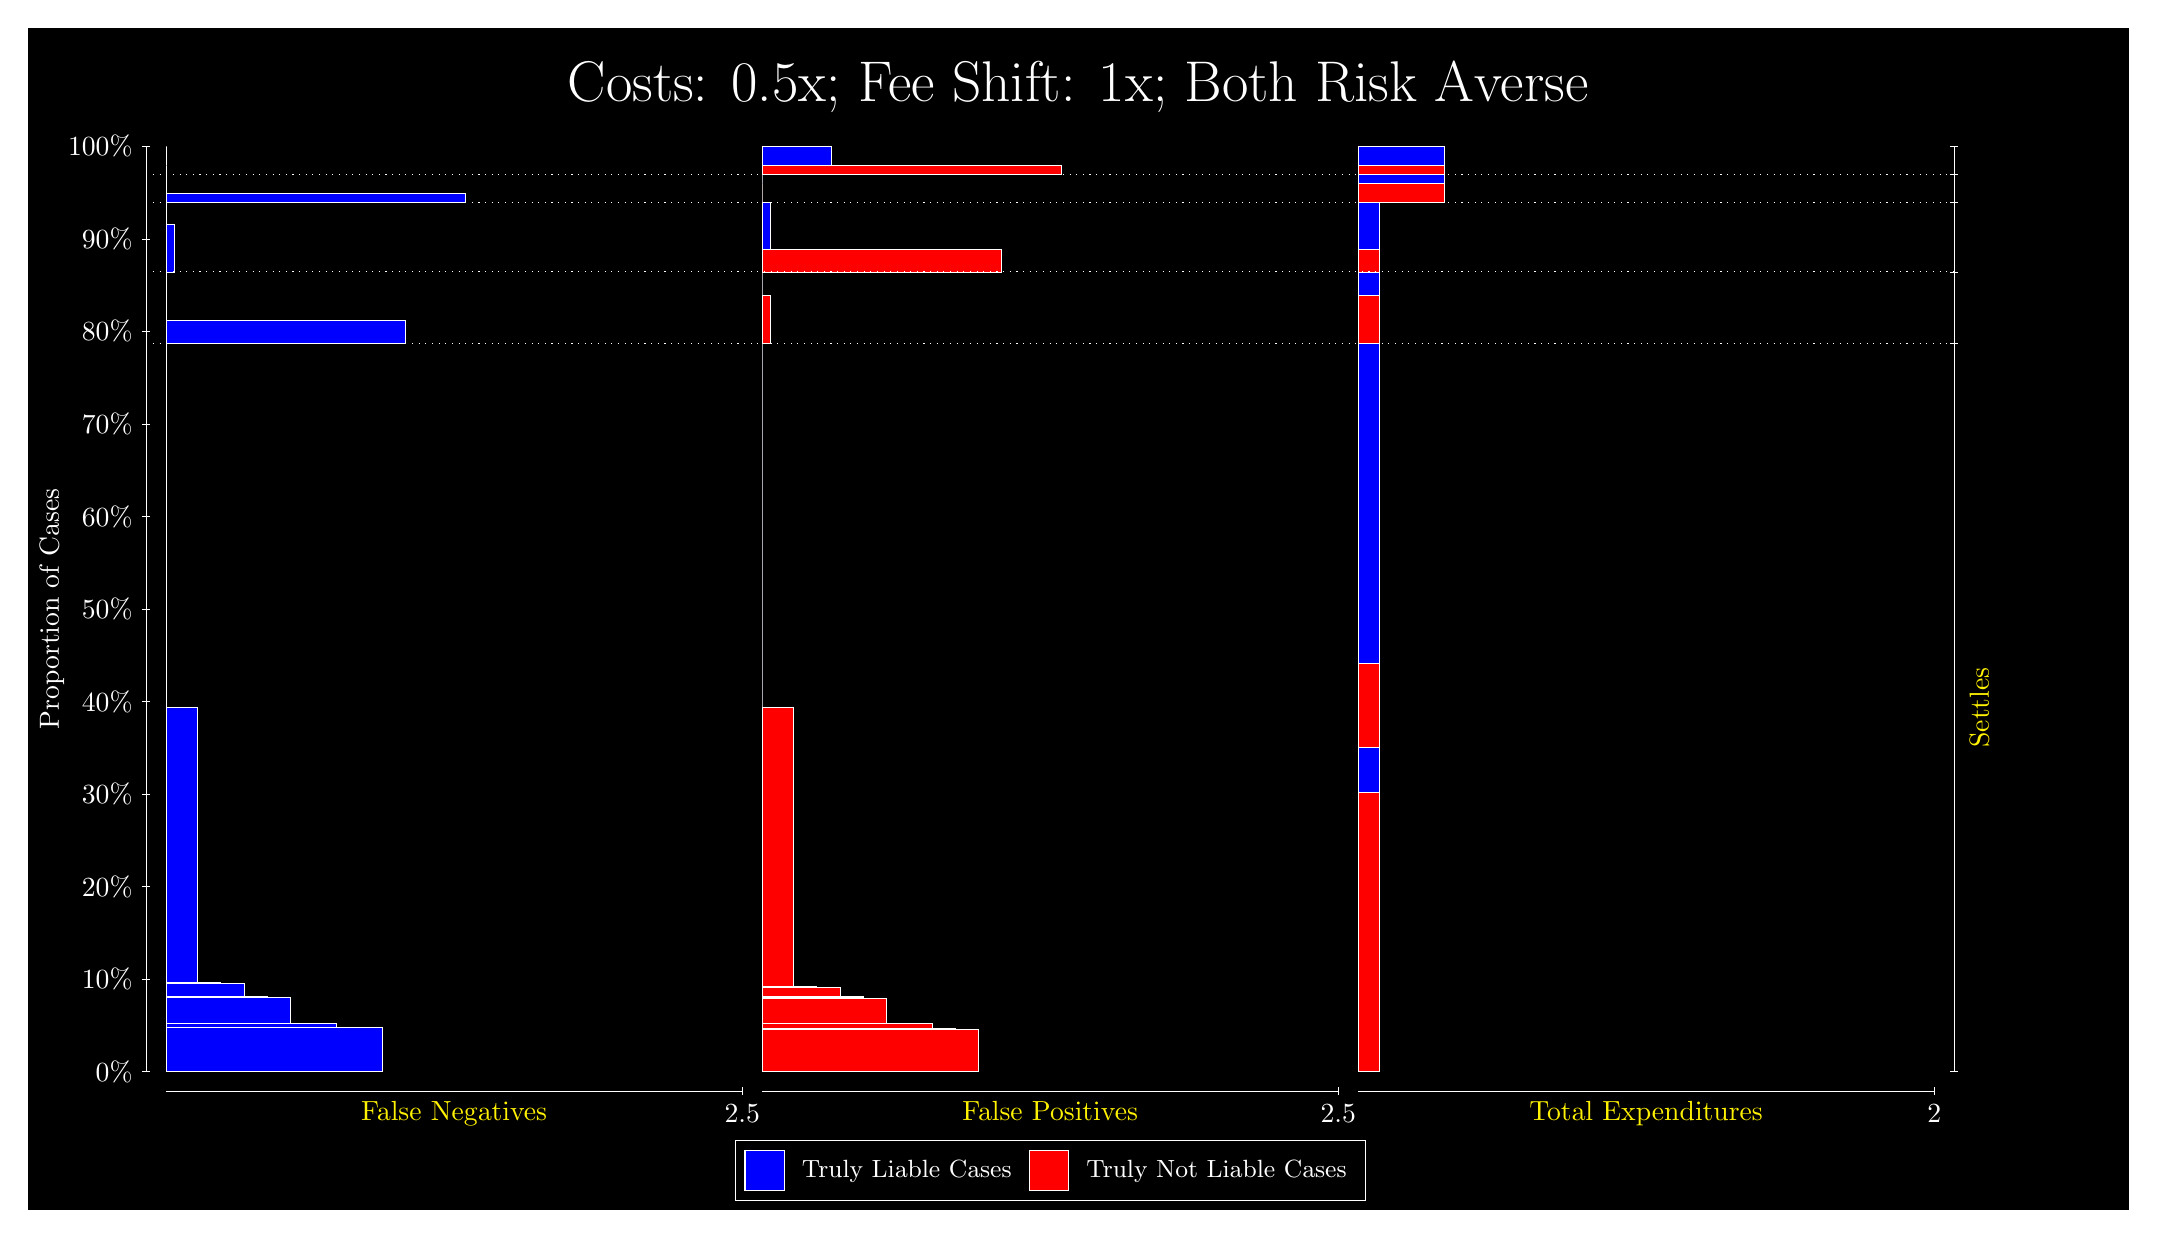
\begin{tikzpicture}
\draw[fill=black] (0,0) rectangle (26.667,15);
\draw[text=white] (0,13.5) rectangle (26.667,15) node[midway] {\huge Costs: 0.5x; Fee Shift: 1x; Both Risk Averse};
\draw[white, very thin] (1.5,1.75) -- (1.5,13.5);
\node[rotate=90, text=white, anchor=center] at (0.3, 7.625) {Proportion of Cases};
\draw[white, very thin] (1.45,1.75) -- (1.55,1.75);
\node[text=white, anchor=east] at (1.45, 1.75) {0\%};
\draw[white, very thin] (1.45,2.925) -- (1.55,2.925);
\node[text=white, anchor=east] at (1.45, 2.925) {10\%};
\draw[white, very thin] (1.45,4.1) -- (1.55,4.1);
\node[text=white, anchor=east] at (1.45, 4.1) {20\%};
\draw[white, very thin] (1.45,5.275) -- (1.55,5.275);
\node[text=white, anchor=east] at (1.45, 5.275) {30\%};
\draw[white, very thin] (1.45,6.45) -- (1.55,6.45);
\node[text=white, anchor=east] at (1.45, 6.45) {40\%};
\draw[white, very thin] (1.45,7.625) -- (1.55,7.625);
\node[text=white, anchor=east] at (1.45, 7.625) {50\%};
\draw[white, very thin] (1.45,8.8) -- (1.55,8.8);
\node[text=white, anchor=east] at (1.45, 8.8) {60\%};
\draw[white, very thin] (1.45,9.975) -- (1.55,9.975);
\node[text=white, anchor=east] at (1.45, 9.975) {70\%};
\draw[white, very thin] (1.45,11.15) -- (1.55,11.15);
\node[text=white, anchor=east] at (1.45, 11.15) {80\%};
\draw[white, very thin] (1.45,12.325) -- (1.55,12.325);
\node[text=white, anchor=east] at (1.45, 12.325) {90\%};
\draw[white, very thin] (1.45,13.5) -- (1.55,13.5);
\node[text=white, anchor=east] at (1.45, 13.5) {100\%};

\draw[white, very thin] (24.457,1.75) -- (24.457,13.5);
\draw[white, very thin] (24.407,1.75) -- (24.507,1.75);
\node[anchor=west] at (24.407, 1.75) {};
\draw[white, very thin] (24.407,10.995) -- (24.507,10.995);
\node[anchor=west] at (24.407, 10.995) {};
\draw[white, very thin] (24.407,11.906) -- (24.507,11.906);
\node[anchor=west] at (24.407, 11.906) {};
\draw[white, very thin] (24.407,12.792) -- (24.507,12.792);
\node[anchor=west] at (24.407, 12.792) {};
\draw[white, very thin] (24.407,13.142) -- (24.507,13.142);
\node[anchor=west] at (24.407, 13.142) {};
\draw[white, very thin] (24.407,13.5) -- (24.507,13.5);
\node[anchor=west] at (24.407, 13.5) {};

\draw[white, very thin, fill=blue] (1.75,1.75) rectangle (4.4946,2.3089);
\draw[white, very thin, fill=blue] (1.75,2.3089) rectangle (4.2018,2.3126);
\draw[white, very thin, fill=blue] (1.75,2.3126) rectangle (3.9091,2.3598);
\draw[white, very thin, fill=blue] (1.75,2.3598) rectangle (3.6163,2.3654);
\draw[white, very thin, fill=blue] (1.75,2.3654) rectangle (3.3236,2.6894);
\draw[white, very thin, fill=blue] (1.75,2.6894) rectangle (3.0308,2.6999);
\draw[white, very thin, fill=blue] (1.75,2.6999) rectangle (2.738,2.8727);
\draw[white, very thin, fill=blue] (1.75,2.8727) rectangle (2.4453,2.8847);
\draw[white, very thin, fill=blue] (1.75,2.8847) rectangle (2.1525,6.3717);
\draw[white, very thin, fill=red] (1.75,6.3717) rectangle (1.75,10.995);
\draw[white, very thin, fill=blue] (1.75,10.995) rectangle (4.7873,11.289);
\draw[white, very thin, fill=red] (1.75,11.289) rectangle (1.75,11.906);
\draw[white, very thin, fill=blue] (1.75,11.906) rectangle (1.8598,12.507);
\draw[white, very thin, fill=red] (1.75,12.507) rectangle (1.75,12.792);
\draw[white, very thin, fill=blue] (1.75,12.792) rectangle (5.5558,12.909);
\draw[white, very thin, fill=red] (1.75,12.909) rectangle (1.75,13.142);
\draw[white, very thin, fill=red] (1.75,13.142) rectangle (1.75,13.258);
\draw[white, very thin, fill=blue] (1.75,13.258) rectangle (1.75,13.5);
\draw[white, very thin, fill=red] (9.3189,1.75) rectangle (12.063,2.2885);
\draw[white, very thin, fill=red] (9.3189,2.2885) rectangle (11.771,2.293);
\draw[white, very thin, fill=red] (9.3189,2.293) rectangle (11.478,2.3588);
\draw[white, very thin, fill=red] (9.3189,2.3588) rectangle (11.185,2.3637);
\draw[white, very thin, fill=red] (9.3189,2.3637) rectangle (10.892,2.6863);
\draw[white, very thin, fill=red] (9.3189,2.6863) rectangle (10.6,2.687);
\draw[white, very thin, fill=red] (9.3189,2.687) rectangle (10.6,2.7);
\draw[white, very thin, fill=red] (9.3189,2.7) rectangle (10.307,2.8237);
\draw[white, very thin, fill=red] (9.3189,2.8237) rectangle (10.014,2.8333);
\draw[white, very thin, fill=red] (9.3189,2.8333) rectangle (9.7214,6.3733);
\draw[white, very thin, fill=blue] (9.3189,6.3733) rectangle (9.3189,10.995);
\draw[white, very thin, fill=red] (9.3189,10.995) rectangle (9.4287,11.612);
\draw[white, very thin, fill=blue] (9.3189,11.612) rectangle (9.3189,11.906);
\draw[white, very thin, fill=red] (9.3189,11.906) rectangle (12.356,12.192);
\draw[white, very thin, fill=blue] (9.3189,12.192) rectangle (9.4287,12.792);
\draw[white, very thin, fill=red] (9.3189,12.792) rectangle (9.3189,13.025);
\draw[white, very thin, fill=blue] (9.3189,13.025) rectangle (9.3189,13.142);
\draw[white, very thin, fill=red] (9.3189,13.142) rectangle (13.125,13.258);
\draw[white, very thin, fill=blue] (9.3189,13.258) rectangle (10.197,13.5);
\draw[white, very thin, fill=red] (16.888,1.75) rectangle (17.162,5.2996);
\draw[white, very thin, fill=blue] (16.888,5.2996) rectangle (17.162,5.8622);
\draw[white, very thin, fill=red] (16.888,5.8622) rectangle (17.162,6.9359);
\draw[white, very thin, fill=blue] (16.888,6.9359) rectangle (17.162,10.995);
\draw[white, very thin, fill=red] (16.888,10.995) rectangle (17.162,11.612);
\draw[white, very thin, fill=blue] (16.888,11.612) rectangle (17.162,11.906);
\draw[white, very thin, fill=red] (16.888,11.906) rectangle (17.162,12.192);
\draw[white, very thin, fill=blue] (16.888,12.192) rectangle (17.162,12.792);
\draw[white, very thin, fill=red] (16.888,12.792) rectangle (17.986,13.025);
\draw[white, very thin, fill=blue] (16.888,13.025) rectangle (17.986,13.142);
\draw[white, very thin, fill=red] (16.888,13.142) rectangle (17.986,13.258);
\draw[white, very thin, fill=blue] (16.888,13.258) rectangle (17.986,13.5);
\draw[white, dotted] (1.5,10.995) -- (24.457,10.995);
\draw[white, dotted] (1.5,11.906) -- (24.457,11.906);
\draw[white, dotted] (1.5,12.792) -- (24.457,12.792);
\draw[white, dotted] (1.5,13.142) -- (24.457,13.142);
\draw[white, very thin] (1.75,1.5) -- (9.0689,1.5);
\node[text=yellow, anchor=north] at (5.4094, 1.5) {False Negatives};
\draw[white, very thin] (9.0689,1.45) -- (9.0689,1.55);
\node[text=white, anchor=north] at (9.0689, 1.45) {2.5};

\draw[white, very thin] (9.3189,1.5) -- (16.638,1.5);
\node[text=yellow, anchor=north] at (12.978, 1.5) {False Positives};
\draw[white, very thin] (16.638,1.45) -- (16.638,1.55);
\node[text=white, anchor=north] at (16.638, 1.45) {2.5};

\draw[white, very thin] (16.888,1.5) -- (24.207,1.5);
\node[text=yellow, anchor=north] at (20.547, 1.5) {Total Expenditures};
\draw[white, very thin] (24.207,1.45) -- (24.207,1.55);
\node[text=white, anchor=north] at (24.207, 1.45) {2};

\node[text=yellow, centered, rotate=90] at (24.777, 6.3725) {Settles};





\draw (12.978300999999998,1.5) node[draw=none] (baseCoordinate) {};
\begin{scope}[align=center]
        \matrix[scale=0.5, draw=white, below=0.5cm of baseCoordinate, nodes={draw}, column sep=0.1cm]{
            \node[rectangle, draw, minimum width=0.5cm, minimum height=0.5cm, fill=blue] {}; &
            \node[draw=none, font=\small, text=white] (B) {Truly Liable Cases}; &
            \node[rectangle, draw, minimum width=0.5cm, minimum height=0.5cm, fill=red] {}; &
            \node[draw=none, font=\small, text=white] (B) {Truly Not Liable Cases}; \\
            };
\end{scope}

\end{tikzpicture}
\end{document}